% !TEX root =  master.tex
\chapter{Evaluation des Kubernetes Prototyps}
\label{Evaluation_K8s}
In den folgenden Unterkapiteln erfolgt das Testen der Funktionsweise des auf dem Kubernetes Cluster bereitgestellten Prototypen. Zudem werden mit Hilfe der bei der Umsetzung des Prototyps gesammelten Erfahrungen und den Ergebnissen der theoretischen Untersuchung der Prototyp und Kubernetes selbst evaluiert.
\section{Testen des Kubernetes Prototyps mittels API-Calls}
Um die vollständige Funktionalität der bereitgestellten Microservices zu testen, wurden die bereits vorhandenen Integrationstests der Microservices durchgeführt. Diese wurden mittels des internen Test-Frameworks gegen die \ac{API}-Endpunkte der Microservices ausgeführt. Dabei wurde unter anderem auch die Service-to-Service Kommunikation getestet, da der Rater-Microservice für einige der ausgeführten Integrationstests vom Business-Config-Microservice abhängig ist.\\
Insgesamt wurden alle Integrationstest erfolgreich ausgeführt, sodass die Funktionalität des bereitgestellten Prototyps auf dem Kubernetes Cluster bestätigt werden kann.
\section{Bewertung der prototypischen Infrastrukturlösung}
\label{bewertung_k8s_prototyp}
Die Evaluation der prototypischen Bereitstellung der SAP Subscription Billing Lösung in einem Kubernetes Cluster erfolgt, wie auch die Evaluation der aktuellen Infrastrukturlösung, mit Hilfe der in Kapitel \ref{kapitel_merkmale_vorgehensweise} definierten Vergleichsmerkmale und Vorgehensweise.
\begin{description}
\item[Performance] \hfill \\
	Bei der Messung der Performance des Kubernetes Clusters wurde die gleiche \ac{HTTP}-Anfrage, welche auch zur Evaluation der \ac{CF}-Plattform eingesetzt wurde, verwendet. Das gesamte Testsetup ist im Anhang in Kapitel \ref{anhang_performancetests} zu finden. Bei der Evaluation des Kubernetes Prototypen wurden, die in der Tabelle \ref{tabelle_performance_k8s} dargestellten Durchschnittswerte ermittelt.
	\begin{table}[ht]
		\centering
		\begin{tabular}[h]{c|c|c|c}
			Threads & Anzahl Anfragen & Antwortzeit pro Anfrage & Durchsatz pro Sekunde \\
			\hline
			100 & 330717,4 & 88,6 ms & 1095,60 
			\\
			\hline
			150 & 305489,4 & 144,4 ms & 1145,85
			\\
			\hline
			200 & 312006,2 & 188,8 ms & 1020,78
			\\
		\end{tabular}\\
	\caption{Ergebnisse Performancetets: Kubernetes Cluster in Belgien}
	\label{tabelle_performance_k8s}
	\end{table}
	\\
	Eine erweiterte Darstellung aller einzelnen Testläufe mit zusätzlichen Variablen ist im Anhang in Kapitel \ref{section_performance_k8s_gardener} und \ref{section_performance_k8s_con_cloud} zu finden.\\
	Da die dabei ermittelten Durchschnittswerte unerwartet schlechter als die in Kapitel \ref{bewertung_cf} dargestellten Ergebnisse der \ac{CF} gewesen sind, wurden zusätzliche Performancetests auf einem weiteren Kubernetes Cluster durchgeführt. Dabei wurde der Rater-Microservice auf dem abteilungsinternen Kubernetes Cluster, das bereits in Kapitel \ref{Konzeption_integration_ci_cd_pipeline} erwähnt wurde, bereitgestellt. Dabei wurden folgende Durchschnittswerte ermittelt.
	\begin{table}[ht]
		\centering
		\begin{tabular}[h]{c|c|c|c}
			Threads & Anzahl Anfragen & Antwortzeit pro Anfrage & Durchsatz pro Sekunde \\
			\hline
			100 & 387270,4 & 75,6 ms & 1290,33 
			\\
			\hline
			150 & 371185,4 & 118,6 ms & 1234,62
			\\
			\hline
			200 & 339434,6 & 173,6 ms & 1127,37
			\\
		\end{tabular}\\
		\caption{Ergebnisse Performancetets: Kubernetes Cluster in Frankfurt}
	\end{table}
	\\
	Die dabei ermittelten Testergebnisse bestätigten die Vermutung, dass die unterschiedliche Performance zwischen der \ac{CF} und dem mittels Gardener provisionierten Kubernetes Cluster hauptsächlich durch die Latenzunterschiede begründet werden können.	Der Latenzunterschied erklärt sich anhand der Verwendung der unterschiedlichen Infrastrukturen. Dabei basiert die \ac{CF} auf der \ac{AWS}-Infrastruktur in einem Rechenzentrum in Frankfurt, wohingegen das für den Prototyp verwendete Kubernetes Cluster aus Kostengründen in einem der \ac{GCP}-Rechenzentren in Belgien betrieben wird.
	\\
	\begin{figure}[h]
		\begin{center}
			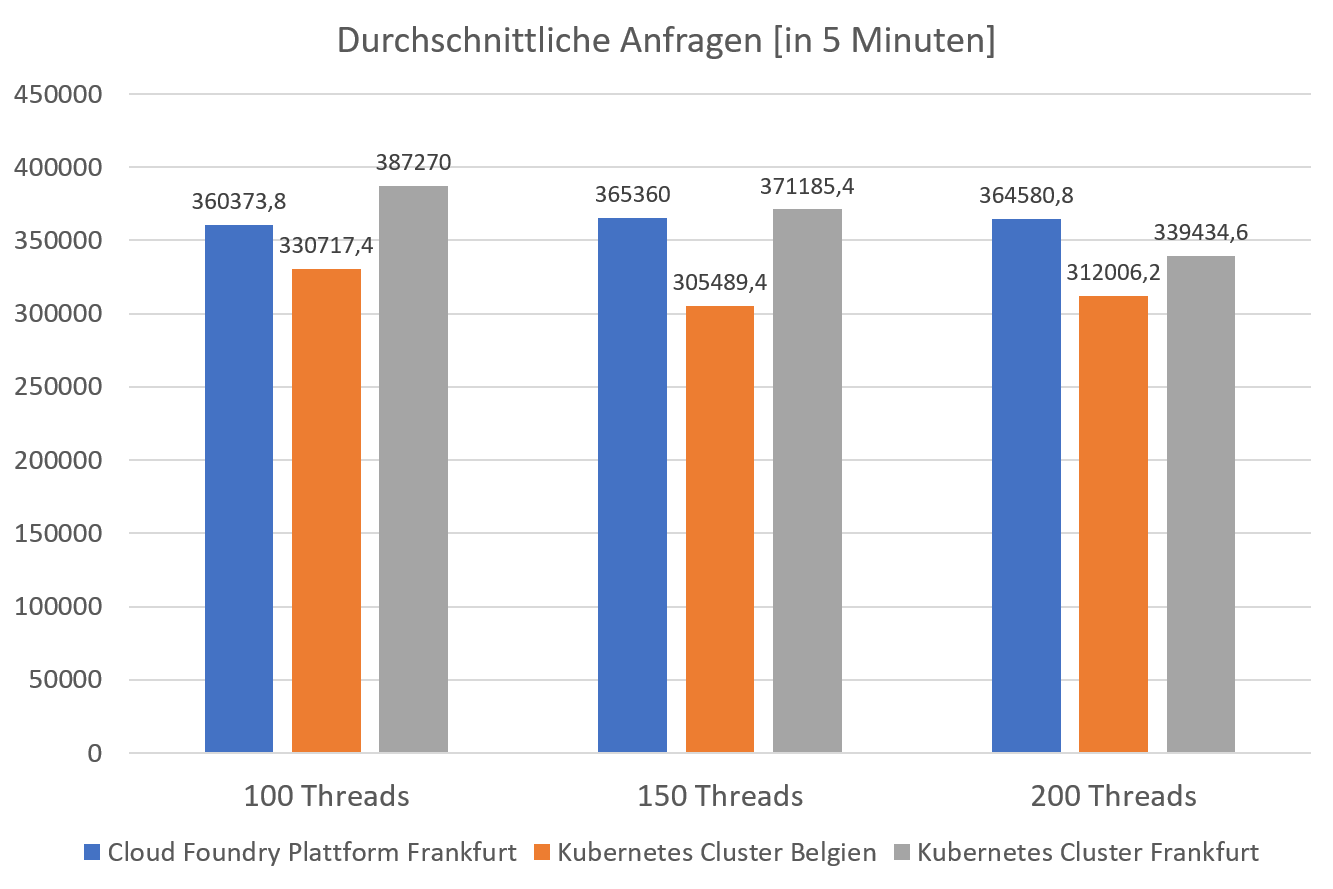
\includegraphics[width=13cm]{img/Performance_Response_Amount.PNG}
			\caption[Ergebnisse Performancetests: Anzahl beantworteter Anfragen]{Ergebnisse Performancetests: Anzahl beantworteter Anfragen}
			\label{performance_anzahl_antworten}
		\end{center}
	\end{figure}
	\begin{figure}[h]
		\begin{center}
			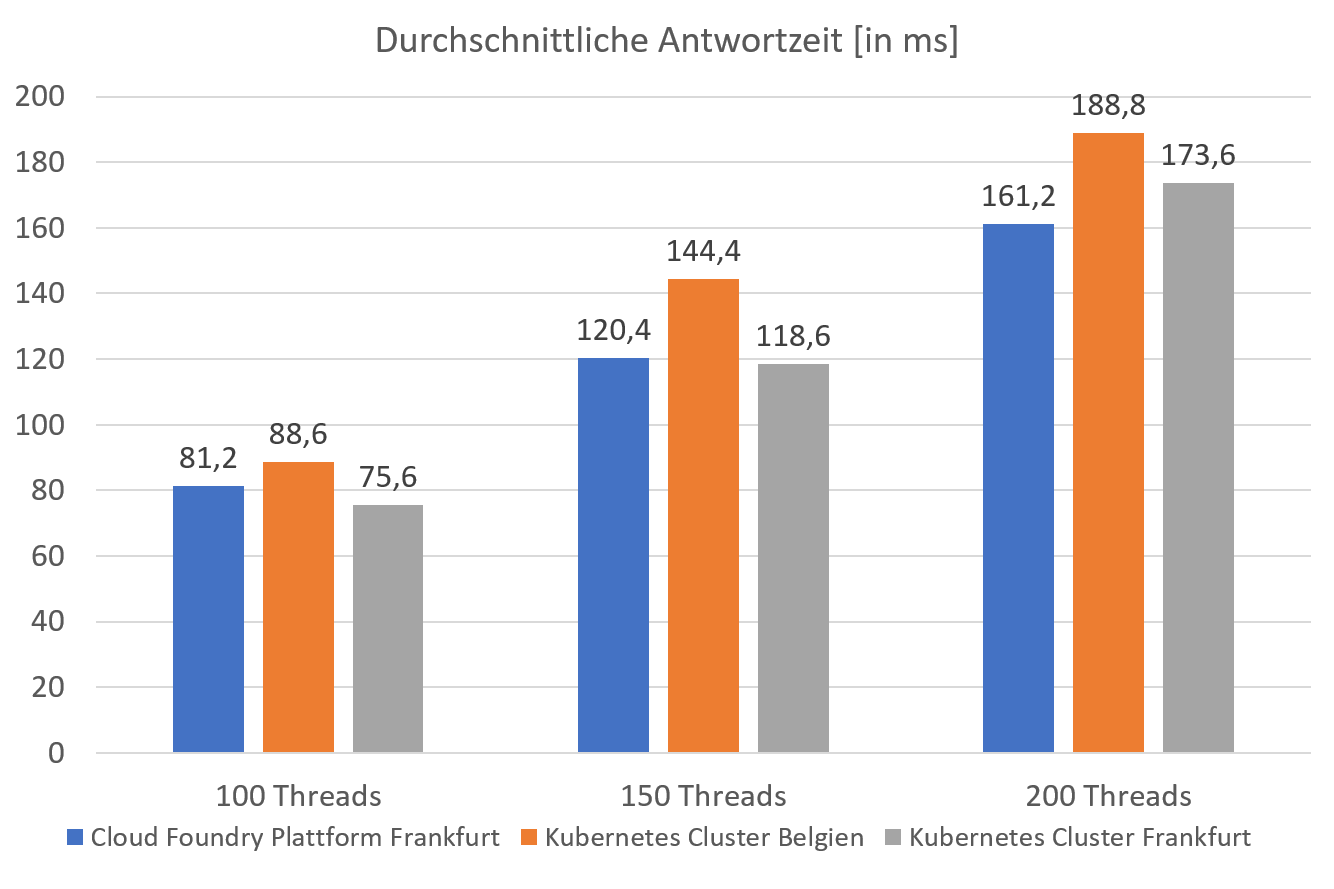
\includegraphics[width=13cm]{img/Performance_Response_Time.PNG}
			\caption[Ergebnisse Performancetests: Durchschnittliche Antwortzeit der Anfragen]{Ergebnisse Performancetests: Durchschnittliche Antwortzeit der Anfragen}
			\label{performance_antwortzeit}
		\end{center}
	\end{figure}
	\\
	%Anmerkung: Siehe Abstand Formattierung
	Das zusätzlich verwendete Cluster wurde ausgewählt, da es ebenfalls in Frankfurt betrieben wird und somit eine bessere Vergleichbarkeit mit der \ac{CF} besteht.\\
	Wie den Abbildungen \ref{performance_anzahl_antworten} und \ref{performance_antwortzeit} zur Gegenüberstellung der Ergebnisse der Performancetests der unterschiedlichen Plattformen und Kubernetes Clustern zu entnehmen ist, gibt es grundsätzlich keine bemerkenswerte Performanceunterschiede zwischen der \ac{CF} und Kubernetes. Dabei konnte \ac{CF} besonders bei einer höheren Anzahl an parallelisierten Anfragen besser als das Kubernetes Cluster abschneiden. Wohingegen der auf dem Kubernetes Cluster bereitgestellte Rater-Microservice bei einer geringeren Anzahl an parallelisierten Anfragen eine geringere durchschnittliche Antwortzeit pro Anfrage und somit eine bessere Performance als der auf der \ac{CF} bereitgestellte Rater-Microservice aufzeigte.\\
\item[Kosten] \hfill \\
	Da Kubernetes und das Gardener Projekt Teil der Open Source Community sind, fallen hierfür keine generellen Servicekosten an. Die für den Betrieb des Kubernetes Clusters anfallenden Kosten setzen sich somit ausschließlich aus den Kosten des \ac{IaaS}-Providers zusammen. Dies sind bei der Verwendung des \ac{GCP} Kosten für die \acsp{VM}, für die persistenten Datenspeicher sowie für die benötigten Load Balancer.\\
	Jedoch werden im Rahmen des Kostenvergleiches der vorliegenden Thesis aus Gründen der Vergleichbarkeit explizit die Kosten für die Application Runtime verwendet.\\
	Dabei können bei der \ac{GCP} folgende sich an die Vergleichswerte von 34 und 780 \ac{GB} \ac{RAM} annähernden Konstellationen eingesetzt werden.\\
	$\textrm{Monatliche Kosten 33,75 \ac{GB} \ac{RAM}:}\\
	= 1 \textrm{x n1-standard-8} + 1 \textrm{x n1-standard-1} \\
	= 30 \textrm{ \ac{GB} \ac{RAM}} + 3,75 \textrm{ \ac{GB} \ac{RAM}}\\
	= 227,27\textrm{\euro} + 28,40\textrm{\euro} = 255,67\textrm{\euro}\\
	\\
	\textrm{Monatliche Kosten 780 \ac{GB} \ac{RAM}:}\\
	= 2 \textrm{x n1-standard-96} + 1 \textrm{x n1-standard-16} \\
	= 720 \textrm{ \ac{GB} \ac{RAM}} + 60 \textrm{ \ac{GB} \ac{RAM}}\\
	= 5458,73\textrm{\euro} + 454,89\textrm{\euro} = 5913,62\textrm{\euro}\\$	
	\\
	Die für die Berechnung verwendeten Kostenangaben stammen von der offiziellen Kostenübersicht der \ac{GCP}.\footnote{Zur Kostenberechnung der \ac{GCP}: \url{https://cloud.google.com/products/calculator/\#&id=f50cd85a-403a-42de-b5dd-fce73f42ecd0}} Da das Angebot der \ac{GCP} nicht mit dem genauen Angebot der \ac{SCP} übereinstimmt, wurden die annähernden Vergleichswerte von 33,75 \ac{GB} \ac{RAM} und 780 \ac{GB} \ac{RAM} gewählt.
	Jedoch ist hierbei zu beachten, dass es sich, anders als bei der \ac{CF}-Umgebung der \ac{SCP}, nicht um feste monatliche Kosten, sondern um ein Pay-Per-Usage-Kostenmodell handelt.\\ 
	Wie bereits in Kapitel \ref{theorie_saas} beschrieben, hat dieses Kostenmodell den großen Vorteil, dass man als Benutzer der Dienste der \ac{GCP} ausschließlich für den tatsächlichen Verbrauch an Rechenressourcen zahlen muss.\\
	Zusätzlich fallen für das Logging des umgesetzten Prototyps keine generellen Servicekosten an, wie es bei der \ac{SCP} der Fall ist. Allerdings muss hierbei beachtet werden, dass der eigens bereitgestellte ELK Stack Rechenressourcen des Clusters konsumiert.\\
\item[Sicherheit] \hfill \\
Im Bereich der Sicherheit zeichnet sich Kubernetes besonders durch das standardmäßige Nichtvorhandensein von extern verfügbaren Endpunkten aus. 
Die auf dem Kubernetes Cluster bereitgestellten Anwendungen und Services sind, wenn nicht explizit gewünscht, ausschließlich im internen Netzwerk des Clusters verfügbar und es existiert keine extern verfügbare \ac{IP}-Adresse.\\
Ein weiterer Sicherheitsaspekt konnte durch die clusterweite Verwendung von \ac{mTLS} erreicht werden. Damit ist die gesamte Kommunikation sowie die Übertragung von Daten abgesichert und verschlüsselt. Zudem ist eine Kommunikation der Microservices ausschließlich nach der erfolgreichen Authentifikation möglich.\autocite[Vgl.][]{IstioAuthors.20200106} \\
\newpage
Die für die \ac{mTLS}-Verschlüsselung benötigten Zertifikate und Tokens werden automatisch bei der Bereitstellung einer Anwendung in einem Istio aktivierten Namespace generiert. Diese werden unter Zuhilfenahme von Kubernetes Secrets im entsprechenden Namespace abgelegt.\\
Des Weiteren wurde, wie in Kapitel \ref{Umsetzung_Landschaften} beschrieben, mit Hilfe von Network Policies die nicht vorgesehene Kommunikation zwischen Microservices komplett unterbunden. Dadurch können ausschließlich die explizit in den Network Policies definierten Microservices miteinander kommunizieren. Auch die Isolation der Namespaces konnte mit den Network Policies erfolgreich umgesetzt werden, sodass keine ungewollte Kommunikation zwischen Microservices aus unterschiedlichen Namespaces stattfinden kann. Zusätzlich wurden die Zugriffe auf die jeweiligen Datenbanken ausschließlich für die vorgesehenen Microservices eingeschränkt. Damit konnte die zusätzliche Absicherung der Datenbanken erfolgreich umgesetzt werden.\\
Die clusterinternen Konfigurationen, wie beispielsweise die Zugangsdaten für die Image Registry, wurden mit Secrets verschlüsselt im Cluster hinterlegt und somit auch abgesichert.\\
Der Kubernetes \ac{API}-Server wird durch die folgende Sicherheitsvorkehrungen geschützt. Der Zugriff kann zum einen von der \textbf{kubectl} \ac{CLI}, von Kubernetes-Objekten selbst oder auch von externen \ac{REST}-Anfragen erfolgen. Dabei wird die Authentifikation und Autorisierung mittels \textbf{User Accounts} und \textbf{Service Accounts} durchgeführt. User Accounts werden für die Benutzer des Kubernetes Clusters verwendet. Hierbei sollte beachtet werden, dass diese innerhalb des Clusters global gültig sind, weshalb hierfür eine eindeutige Bezeichnung gewählt werden sollte. Service Accounts werden hingegen für die Authentifikation und Autorisierung der eigentlichen Prozesse der Pods eingesetzt. Diese sind hingegen spezifisch einem Namespace zugeordnet.\autocite[Vgl.][]{KubernetesAuthors.20190506}
\\
Der externe Zugriff eines Benutzers wird durch die Verwendung der \ac{CLI} mit Hilfe des benötigten Root-Zertifikates authentifiziert. Dieses ist normalerweise in der lokalen Kubernetes Konfigurationsdatei gespeichert. Im Fall der Provisionierung des Clusters mit Gardener kann dieses direkt aus dem eigenen Gardener Dashboard heruntergeladen werden.\autocite[Vgl.][]{KubernetesAuthors.20191106}\\
Innerhalb des Clusters sind die Sicherheitsmechanismen des \ac{API}-Servers durch die \ac{RBAC} umgesetzt. Dabei werden interne Rollen angelegt, welche unterschiedliche Berechtigungen haben. Eine solche kann beispielsweise eine Berechtigung mit einem ausschließlich lesenden Zugriff auf die in einem Namespace vorhandenen Secrets sein. Die Rollen werden mit \textbf{Role Bindings} an die Benutzer des Clusters gebunden.\autocite[Vgl.][]{KubernetesAuthors.20191023}\\
Somit können mit der \ac{RBAC} umfangreiche Berechtigungskonzepte umgesetzt werden. Jedoch ist zu erwähnen, dass im Rahmen der prototypischen Portierung kein Berechtigungskonzept umgesetzt worden ist, da ausschließlich der Autor der vorliegenden Thesis Zugriff auf das Kubernetes Cluster hatte.\\
\item[Verfügbarkeit] \hfill \\
Grundsätzlich ist die Verfügbarkeit des Kubernetes Clusters ausschließlich von der Verfügbarkeit der Infrastruktur abhängig. Im Fall des umgesetzten Prototyps gibt die \ac{GCP} laut \ac{SLA} aktuell eine Verfügbarkeit der virtuellen Maschinen von mindestens 99,99\% pro Monat an.\autocite[Vgl.][]{GoogleCloudAuthors.20200113}\\
\\
Für die Sicherstellung der clusterinternen Verfügbarkeit der bereitgestellten Anwendungen bietet Kubernetes folgende Mechanismen und \ac{API}-Objekte an.\\ 
Durch die Verwendung von \textbf{Liveness Probes}, \textbf{Startup Probes} und \textbf{Readiness Probes} kann jeweils das generelle Vorhandensein der Anwendungsbereitstellung, das erfolgreiche Starten als auch die Funktionalität der Anwendung überprüft werden. Hierbei können die Proben als \ac{HTTP}- oder \ac{TCP}-Anfragen umgesetzt werden. Eine weitere Möglichkeit zur Überprüfung des Status ist das Ausführen von Kommandos innerhalb des bereitgestellten Containers.\\
Im Vergleich zu \ac{CF} sind die umfangreichen Konfigurationsmöglichkeiten der von Kubernetes angebotenen Proben durchaus hervorzuheben. Mit der Konfigurationseinstellung \textbf{initialDelaySeconds} kann beispielsweise eine initiale Verzögerung für die Überprüfung des Anwendungsstatus, mit den \textbf{timeoutSeconds} die genaue Timeoutzeit der Proben oder mit \textbf{failureThreshold} die maximale Anzahl an Neustarts des Pods konfiguriert werden.\autocite[Vgl.][]{KubernetesAuthors.20200112}\\
\\
Zudem unterstützt Kubernetes das \textbf{Multi Zonen Konzept}, welches zur weiteren Steigerung der Verfügbarkeit dient. Dabei kann ein Cluster in mehreren \textbf{Failure Zones} eines \ac{IaaS}-Providers bereitgestellt werden. Dies bedeutet, dass innerhalb eines Clusters Worker Nodes verwendet werden können, die auf \acsp{VM} aus unterschiedlichen Zonen basieren.\\ 
Der große Vorteil dabei ist, dass bei einem Ausfall einer Zone eines \ac{IaaS}-Providers nicht alle Worker Nodes auf einmal ausfallen. Generell kann dadurch besonders die generelle Resilienz der \ac{SaaS}-Lösung verbessert werden.\\
\newpage
Allerdings sollte bei der Umsetzung des Multi Zonen Konzeptes beachtet werden, dass aus Latenzgründen der Netzwerkkommunikation keine zu sehr voneinander entfernten Zonen in einem Cluster verwendet werden sollten.\autocite[Vgl][]{KubernetesAuthors.20190612}\\
\\
Ein weiteres auf dem Multi Zonen Konzept aufbauendes Projekt ist das \textbf{Cluster Federation Projekt}. Dabei wird das Multi Zonen Konzept um das Ziel der Verwendung mehrerer \ac{IaaS}-Provider erweitert. Vor allem auch On-Premise Cluster sollen dabei unterstützt werden. Dies wird durch die virtuelle Aggregation mehrerer Cluster zu einem einzigen umgesetzt. Das Hauptziel des Cluster Federation Konzeptes ist die Maximierung der Verfügbarkeit. Dies soll beispielsweise durch die Auslagerung von Rechenlast auf ein in der Public-Cloud gehostetes Cluster ermöglichen, falls die Rechenkapazitäten des On-Premise Clusters nicht mehr ausreichen sollten.\autocite[Vgl][]{KubernetesCommunity.20150820}\\
Dennoch muss beachtet werden, dass es sich hierbei um ein Projekt handelt, das in der Version \textbf{v1} veraltet\autocite[Vgl][]{KubernetesAuthors.20191021} und in der Version \textbf{v2} aktuell noch in der Alpha Phase ist.\autocite[Vgl][]{GitHubRepositoryKubernetesSIG.20190815}\\
\item[Skalierbarkeit] \hfill \\
Generell ermöglicht Kubernetes die Skalierbarkeit auf unterschiedlichen Ebenen. Dabei unterstützen zum Beispiel mittels Gardener oder der \ac{GKE} provisionierte Cluster unter anderem die Skalierung auf der gesamten Node-Ebene. Dies bedeutet, dass abhängig von der aktuellen Auslastung der Worker Nodes zusätzliche \acsp{VM}, welche als weitere Worker Nodes dienen, dynamisch bereitgestellt werden können.\autocite[Vgl][]{GitHubRepositoryGardener.20190401}\\
%\footnote{Gardener Node Autoscaler: \url{https://github.com/gardener/autoscaler}}
Bei Gardener kann für die automatische Skalierung auf Worker Node Ebene beispielsweise eine Zielauslastung der \ac{VM}-Instanzen und der Instanztyp angegeben werden. Dabei wird bei einer Überschreitung der Zielauslastung automatisch eine weitere \ac{VM}-Instanz von dem \ac{IaaS}-Provider provisioniert.\autocite[Vgl][]{KubernetesAuthors.20191126}\\
\\
Des Weiteren kann mit Hilfe des \textbf{Horizontal Pod Autoscalers}, welcher auch im Prototyp implementiert worden ist, eine automatische, horizontale Skalierung auf Pod-Ebene umgesetzt werden. Dabei wird vergleichbar mit der Skalierung auf Node-Ebene, bei der Überschreitung der Zielauslastung des Pods ein weiteres Podreplikat generiert.\\
\\
Zusätzlich kann durch das \textbf{Vertical Pod Autoscalers} Projekt auch eine automatische vertikale Skalierung der Pods umgesetzt werden. Dies bedeutet, dass die für die Container der Pods zur Verfügung stehenden Rechenressourcen dynamisch skaliert werden können. Jedoch handelt es sich zum aktuellen Zeitpunkt der Thesis hierbei noch um eine Funktionalität, die sich aktuell noch im Alpha Status befindet und mit einer Custom Ressource Definition implementiert werden muss, weshalb diese innerhalb des Prototyps nicht umgesetzt wurde.\autocite[Vgl][]{GitHubRepositoryKubernetes.20191127}%\footnote{Kubernetes Vertical Pod Autoscaler: \url{https://github.com/kubernetes/autoscaler/tree/master/vertical-pod-autoscaler}}
\\
\item[Konfigurierbarkeit] \hfill \\
Die Erkenntnisse aus der praktischen Umsetzung des Kubernetes Prototyps haben gezeigt, dass Kubernetes im Punkt der Konfigurierbarkeit generell keine Einschränkungen vorsieht.\\
Dabei können alle Objekte des Kubernetes \ac{API}-Servers manuell mit der jeweiligen Manifestdatei oder der \ac{CLI} konfiguriert werden. Besonders die umfangreiche Konfigurierbarkeit der Proben zur Überprüfung der Verfügbarkeit der bereitgestellten Anwendungen erwies sich als hilfreich und konnte einige Probleme lösen, welche bisher innerhalb der aktuellen Infrastrukturlösung aufgetreten sind.\\ Ein Beispiel dafür ist das fehlerhafte Terminieren einer Anwendung bei einer kurzzeitig erhöhten Antwortzeit, obwohl diese eigentlich funktionsfähig gewesen ist. Dieses beispielhafte Problem konnte durch die Erhöhung der Timeoutzeiten bei der Umsetzung des Kubernetes Prototyps gelöst werden.\\
Generell bietet Kubernetes mit den Custom Ressource Definitions die zusätzliche Möglichkeit an, eigene Kubernetes \ac{API}-Objekte zu erstellen und innerhalb des Clusters zu verwenden. Allerdings war dies in der vorliegenden Arbeit nicht notwendig, da alle benötigten Funktionalitäten durch Kubernetes native oder von Istio implementierter \ac{API}-Objekte abgedeckt wurden.\autocite[Vgl.][]{KubernetesAuthors.20191210}\\
\item[Erweiterbarkeit] \hfill \\
Bezüglich der Erweiterbarkeit der bereitgestellten Anwendungen sehen die hierfür benutzten Kubernetes-Objekte mehrere Aktualisierungsstrategien vor.\\
Die für den Prototyp verwendete \textbf{Rolling Update} Strategie ähnelt sehr stark der Blue-Green Deployment Strategie der \ac{CF}. Jedoch unterscheiden sich diese bei der Aktualisierung einer Anwendung, welche mit mehreren Replikationen bereitgestellt ist. Dabei wird in der Rolling Update Strategie jeweils schrittweise die festgelegte Anzahl an Replikation zusätzlich bereitgestellt. 
\newpage
Wenn diese Bereitstellung erfolgreich gewesen ist, wird die gleiche Anzahl an replizierten Pods, welche nicht mehr aktuell sind, terminiert. \\
Dieser Vorgang wird so lange wiederholt, bis alle replizierten Pods schrittweise aktualisiert sind.\\
Generell bietet dies den Vorteil, dass während der Aktualisierung der Anwendung mit mehreren replizierten Pods nicht gleichzeitig alle Podreplikate zusätzlich in der aktualisierten Version bereitgestellt werden müssen. Durch die Verwendung der Rolling Update Strategie können die für die Aktualisierung der Anwendung zusätzlich benötigten Rechenressourcen insgesamt minimiert werden.\\
Zudem kann bei der Verwendung eines Kubernetes Deployments der genaue Prozentsatz an gleichzeitig aktualisierten Pods sowie der hierfür benötigte maximale Ressourcenbedarf konfiguriert werden. Dies erfolgt mittels der Konfiguration der \textbf{maxUnavailable-} und der \textbf{maxSurge}-Einstellung.\autocite[Vgl.][]{KubernetesAuthors.20191122}\\
Insgesamt kann durch die Verwendung der nativen Rolling-Update-Strategie die schrittweise Aktualisierung der Anwendung ohne Unterbrechung des Anwendungsservices durchgeführt werden.\\
Außerdem bietet der Service Mesh Istio, wie bereits in Kapitel \ref{Umsetzung_Landschaften} erläutert, die Möglichkeit des Canary Releasing Szenarios. Dieses kann besonders in Kombination mit der Rolling Update Strategie für Rollback-Szenarien bei einer fehlerhaften Anwendungsaktualisierung genutzt werden. Dabei kann mit Hilfe des Kubernetes Deployment-Objektes bei einer fehlerhaften Aktualisierung die gesamte Anwendungsaktualisierung rückgängig gemacht und zur letzten stabilen Version der Anwendung zurückgesetzt werden.\\
\\
Des Weiteren können mit dem Helm Package Manager zusätzliche, vorkonfigurierte Open Source Tools, wie beispielsweise der implementierte ELK Stack, innerhalb kurzer Zeit und ohne umfangreiche Konfigurationen implementiert werden. Eine Übersicht aller offiziell angebotenen Helm Charts ist unter dem angegeben Link zu finden.\footnote{Übersicht aktuell angebotener Helm Charts: \url{https://hub.helm.sh/}}\\
\item[Einarbeitungszeit] \hfill \\
Besonders die bei der praktischen Arbeit gesammelten Erfahrungen haben gezeigt, dass bei der Verwendung von Kubernetes grundsätzlich mit einer erhöhten Einarbeitungszeit gerechnet werden sollte. Dabei wird vor allem für eine erstmalige Bereitstellung einer Anwendung ein grundlegendes Verständnis der theoretischen Konzepte und den Funktionalitäten der einzelnen \ac{API}-Objekte benötigt.\\
\newpage
Außerdem müssen zum Beispiel für die Service-to-Service-Kommunikation oder auch dem Erstellen eines extern verfügbaren Endpunktes weitere Kubernetes \ac{API}-Objekte konfiguriert und implementiert werden.\\
Besonders mit Hilfe des Einsatzes des Service Meshes Istio wird die Komplexität der Plattform erhöht. Dadurch bedarf es seitens des Administrators der Kubernetes Clusters ein zusätzliches Verständnis für die grundlegenden Konzepte eines Services Meshes und deren spezifische Umsetzung.\\
\item[Portierbarkeit] \hfill \\
Bei der Provisionierung des Kubernetes Clusters mittels Gardener hat sich gezeigt, dass besonders Gardener auf eine umfangreiche Portierbarkeit des Clusters abzielt. Wie in Kapitel \ref{Umsetzung_Provisionierung_Cluster} aufgezählt, unterstützt das Gardener Projekt grundsätzlich eine Vielzahl an \ac{IaaS}-Providern. In Kombination mit dem bereits erläuterten Multi Zone Konzept von Kubernetes oder dem Cluster Federation Projekt ermöglicht dies die Provisionierung eines global verteilten Kubernetes Clusters, welches nicht ausschließlich von einem regionalen Rechenzentrum eines \ac{IaaS}-Providers abhängig ist. Dabei kann die für die Nodes verwendete Infrastruktur von mehreren \ac{IaaS}-Providern aus unterschiedlichen Zonen und auch in Kombination mit On-Premise-Rechenressourcen bereitgestellt werden.\\
Hierbei sollten jedoch vor allem durch die Latenz bedingte Netzwerkprobleme beachtet werden. Außerdem befindet sich das Cluster Federation Projekt zum aktuellen Zeitpunkt der Thesis noch in keiner stabilen Version, weshalb die zuvor genannte Möglichkeit mehr als eine Vision betrachtet und nicht in bereits produktiv eingesetzten Infrastruktur-Landschaften eingesetzt werden sollte.\\
\item[Infrastruktur-Services] \hfill \\
Wie bereits in den einzelnen Unterkapiteln des Kapitels \ref{Umsetzung_K8s_Cluster} erläutert, konnten einige der innerhalb der aktuellen Infrastrukturlösung zusätzlich benötigten Komponenten und Infrastruktur-Services durch die nativen Funktionalitäten von Kubernetes und dem Service Mesh Istio ersetzt werden. Zusammengefasst konnten dabei die benötigte Routingfunktionalität des Landscape Routers anhand der möglichen Routingregeln der Virtual Services von Istio abgedeckt werden.\\
Auch der zentrale Credential Store Vault ist für den umgesetzten Prototyp nicht mehr notwendig, da durch die Verwendung der \ac{mTLS}-Verschlüsselung keine Authentifizierung der Microservices mit Hilfe von Credentials benötigt wird.\\
Die Service Discovery Funktionalitäten des Eureka-Services konnten durch den Einsatz der nativen Kubernetes Services und der automatischen \ac{DNS}-Auflösung von Kubernetes abgedeckt werden. \\
Zusätzlich bietet die Verwendung von Virtual Services weitere Funktionalitäten, wie beispielsweise die in Kapitel \ref{Umsetzung_S2S_Kommunikation} erklärten Failover Szenarien bei einer fehlerhaften Kommunikation zwischen den Microservices.
\\
\item[Monitoring und Loggings] \hfill \\
Innerhalb der praktischen Umsetzung wurden die bisher genutzten Tools für das Monitoring und Logging erfolgreich auch für den Kubernetes Prototyp implementiert.
Dabei ist das Monitoring-Konzept mittels der Integration des Kubernetes Clusters in den vorhandenen Dynatrace-Server gelungen. Dadurch existieren im Bereich des Monitorings des Clusters keine Einschränkungen und die von Dynatrace bereitgestellten Funktionalitäten können vollständig verwendet werden.\\
\\
Auch der ELK Stack konnte erfolgreich auf dem Kubernetes Cluster implementiert werden. Allerdings wurde im Vergleich zum Logging-Service der \ac{SCP} die Komponente Logstash durch Filebeat ersetzt. Allerdings wurden innerhalb der praktischen Evaluation des umgesetzten Loggingkonzeptes keine fehlenden Funktionalitäten festgestellt werden.\\
Zudem sollte beachtet werden, dass für die generelle Verwendung des ELK-Stacks neben den Betriebskosten der Rechenressourcen keine weiteren Servicekosten anfallen. Jedoch wird für den selbst betriebenen ELK-Stack zusätzlicher Aufwand für das Monitoring und die Sicherung und Archivierung der Daten benötigt. 

\end{description}